\section{Estrutura}

O foguete de garrafa, geralmente construído com garrafas PET, é um ótimo projeto educacional didático que engloba diversas áreas de conhecimento, como estruturas, software, energia, eletrônica e até mesmo física. O funcionamento de um foguete de garrafa pode ser explicado pela Terceira Lei Newton: para toda ação, há uma reação igual e oposta. A "ação" neste sistema de propulsão é a expulsão forçada de uma massa de água pelo bocal do foguete, impulsionada pelo ar comprimido injetado no interior da garrafa, que exerce determinada pressão sobre a água, forçando-a para fora em alta velocidade. A "reação" seria a força igual e oposta, chamada de empuxo, que "empurra" o foguete para cima.

\subsection{Estrutura do Foguete}

A estrutura principal do foguete de garrafa é a própria garrafa PET, que serve como fuselagem e, simultaneamente, como câmara pressão para a água e o ar comprimido. A escolha do PET se deu por sua capacidade de suportar altas pressões internas, facilidade de manuseamento e baixo custo para o projeto. Para garantir um voo controlado, o foguete possui alguns elementos extras: a coifa e as aletas. A coifa foi também feita de uma seção cortada de outra garrafa PET e fixada na parte superior para minimizar o atrito do ar e o arrasto durante o lançamento. As aletas serão explicadas ao longo deste relatório. A escolha dos materiais, design e integração, demonstram como várias vertentes da engenharia se unem para construir um projeto funcional e eficiente.

Em adição à estrutura do foguete, houve a integração um sistema eletrônico, posicionado na coifa. A decisão de sua localização foi tomada por dois fatores: adição de massa na coifa que, mesmo sendo baixa, auxiliaria na estabilidade do voo e, adicionalmente, seria mais seguro para os componentes. Para garantir que o impacto da descida não danificasse o sistema, foi criado uma estrutura de isopor que se encaixava com módulo eletrônico, dessa forma ele não seria movimentado, além disso, mais acima adicionamos uma grande esponja, com o intuito de amenizar a colisão. Todas as peças alocadas na coifa possuem baixa massa, fazendo com que o voo não fosse muito estável, portanto, foi decido adicionar pequenas pedras no topo, trazendo mais controle na trajetória do lançamento. 

\begin{figure}[H]
	\centering
	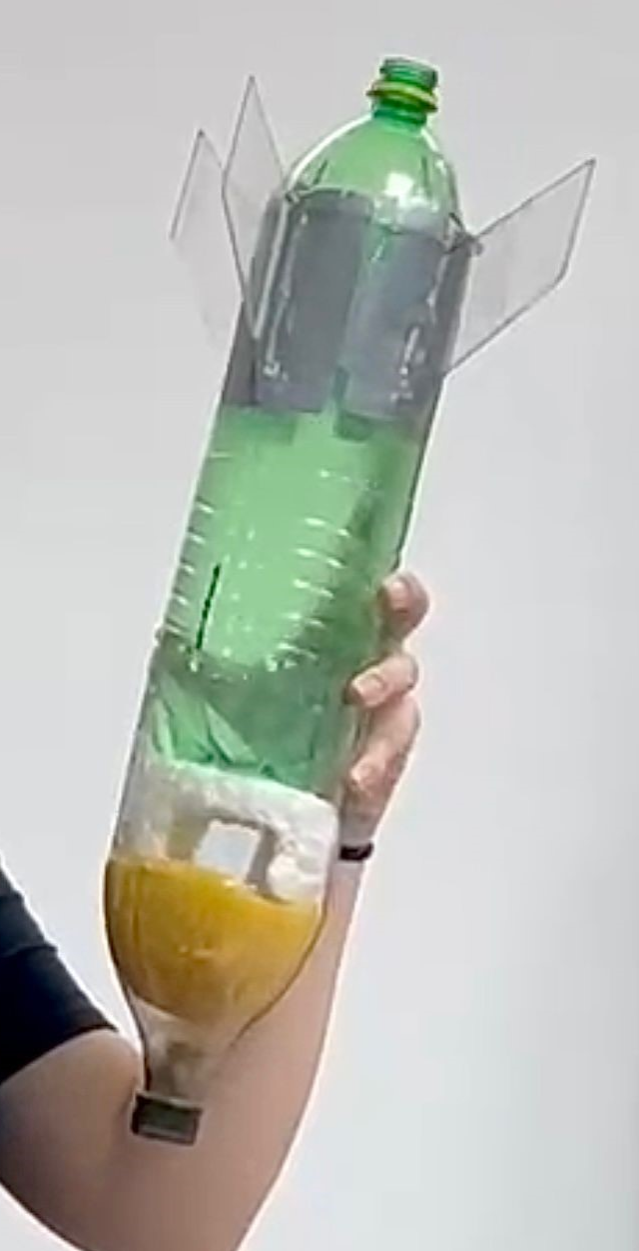
\includegraphics[width=0.5\textwidth,height=\textheight,keepaspectratio]{figuras/estruturas/foguete_foto.png}
	\caption{Foguete usado no dia de lançamento.}
	\label{fig_foguete_lancamento}
\end{figure}

\subsection{Base de Lançamento}

A concepção da base priorizou a estabilidade como um critério fundamental para garantir a precisão e a segurança das operações. A escolha por uma configuração com base de apoio quadrada, em detrimento de geometrias alternativas como a de tripé, é justificada por princípios da estática. A geometria quadrada proporciona uma área de contato com o solo significativamente maior, otimizando a distribuição das cargas e minimizando a suscetibilidade ao tombamento, mesmo sob a influência de perturbações externas, como o impulso do lançamento. Em contrapartida, uma estrutura do tipo tripé, embora apresente estabilidade em superfícies irregulares, possui uma área de projeção menor, tornando-a mais vulnerável a momentos fletores induzidos por forças laterais. Para elevar ainda mais a estabilidade, o projeto final integrou esta estrutura de PVC a uma fundação de madeira, composta por MDF na face superior e compensado nas outras, como consta na Fig. 2. Esta adaptação combina a geometria estável do PVC com a massa e a ampla área de contato da fundação, garantindo resistência a deslocamentos e vibrações.

\begin{figure}[H]
	\centering
	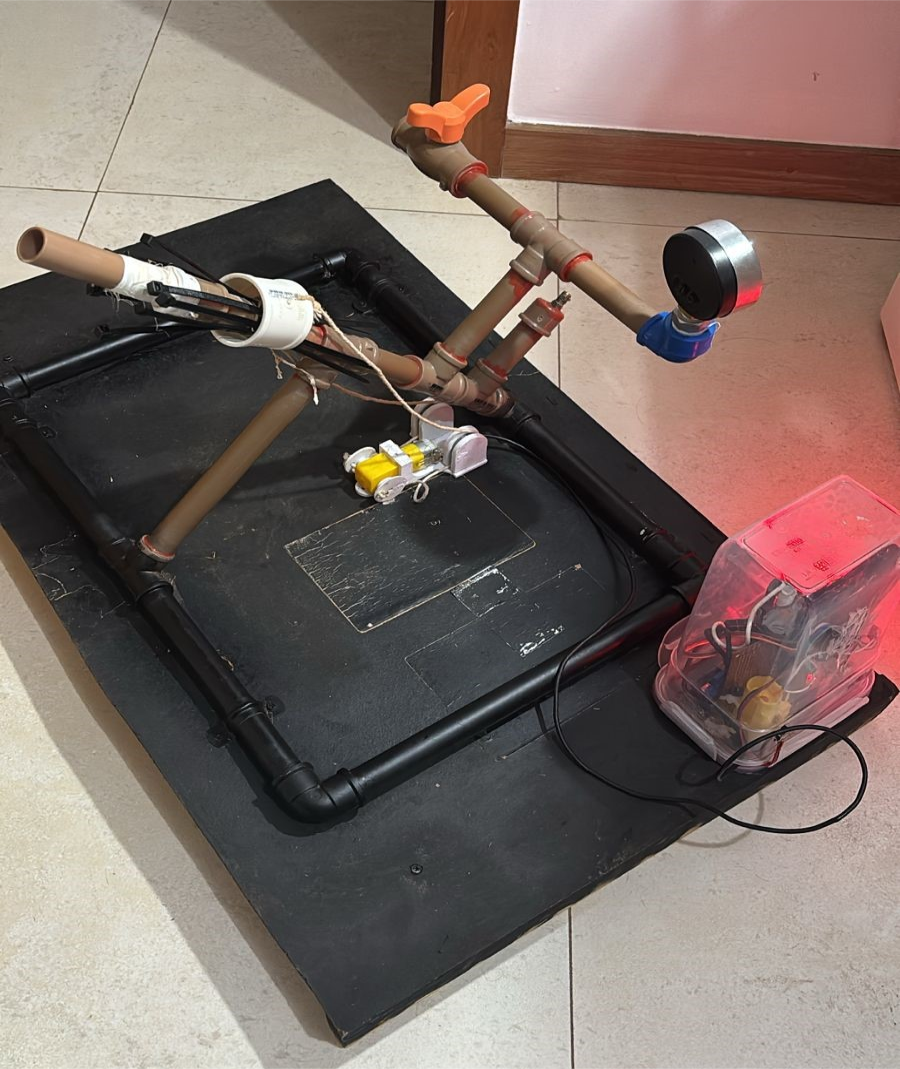
\includegraphics[width=0.75\textwidth,height=\textheight,keepaspectratio]{figuras/estruturas/base_foguete.png}
	\caption{Visão isométrica da base do foguete usada no dia de lançamento.}
	\label{fig_visao_base}
\end{figure}

Do ponto de vista da mecânica do lançamento, foi adotada a decisão estratégica de fixar o ângulo de lançamento em 45°. Segundo os princípios da mecânica clássica, o alcance de um projétil em um cenário ideal sem resistência do ar é maximizado neste ângulo, conforme a Eq. 1, cuja trajetória parabólica é modelada por funções quadráticas \cite{araujo2023}:

\begin{equation}
R = \frac{V_0 \sin(2\theta)}{g}
\end{equation}

Onde $R$ é o alcance [m], $V_0$ é a velocidade inicial [m/s], $g$ é a aceleração da gravidade [m/s$^2$] e $\theta$ é o ângulo de inclinação [$^\circ$] em relação à base. Estudos anteriores sobre o desenvolvimento de foguetes de garrafa PET corroboram que a otimização dos parâmetros de lançamento é fundamental para o controle da trajetória (COPPOLA; IZOLA, 2017). Assim, a decisão de engenharia de fixar o ângulo visou simplificar a complexidade do problema, eliminando uma variável e permitindo que o controle de alcance para os alvos de 10, 20 e 30 metros fosse focado exclusivamente no ajuste da pressão e do volume de água, o que torna a calibração do sistema mais direta. 

A seleção de materiais foi um processo deliberado, visando um balanço ótimo entre desempenho, custo e facilidade de manufatura. Para a estrutura de pressurização, o Policloreto de Vinila (PVC) foi escolhido por sua notável facilidade de manuseio, baixo custo e resistência à corrosão, sendo um material normatizado para o transporte de água fria sob pressão, o que valida sua aplicação no projeto \cite{tigre_soldavel}. Esta escolha superou alternativas metálicas que, embora mais rígidas, implicariam em maior complexidade de fabricação e custo. Para a fundação, a escolha da madeira foi estratégica: utilizou-se MDF na face superior por sua superfície lisa e densa, ideal para a fixação dos componentes, e compensado nas laterais por sua melhor relação resistência-peso. Por fim, para o case de proteção do servo motor, ilustrado pela Fig. 3, optou-se pelo filamento ABS em vez do PLA. O ABS oferece resistência térmica e a impacto superiores, propriedades cruciais para um componente funcional exposto a condições externas de sol e possíveis impactos \cite{ozsoy2021}.

\begin{figure}[H]
	\centering
	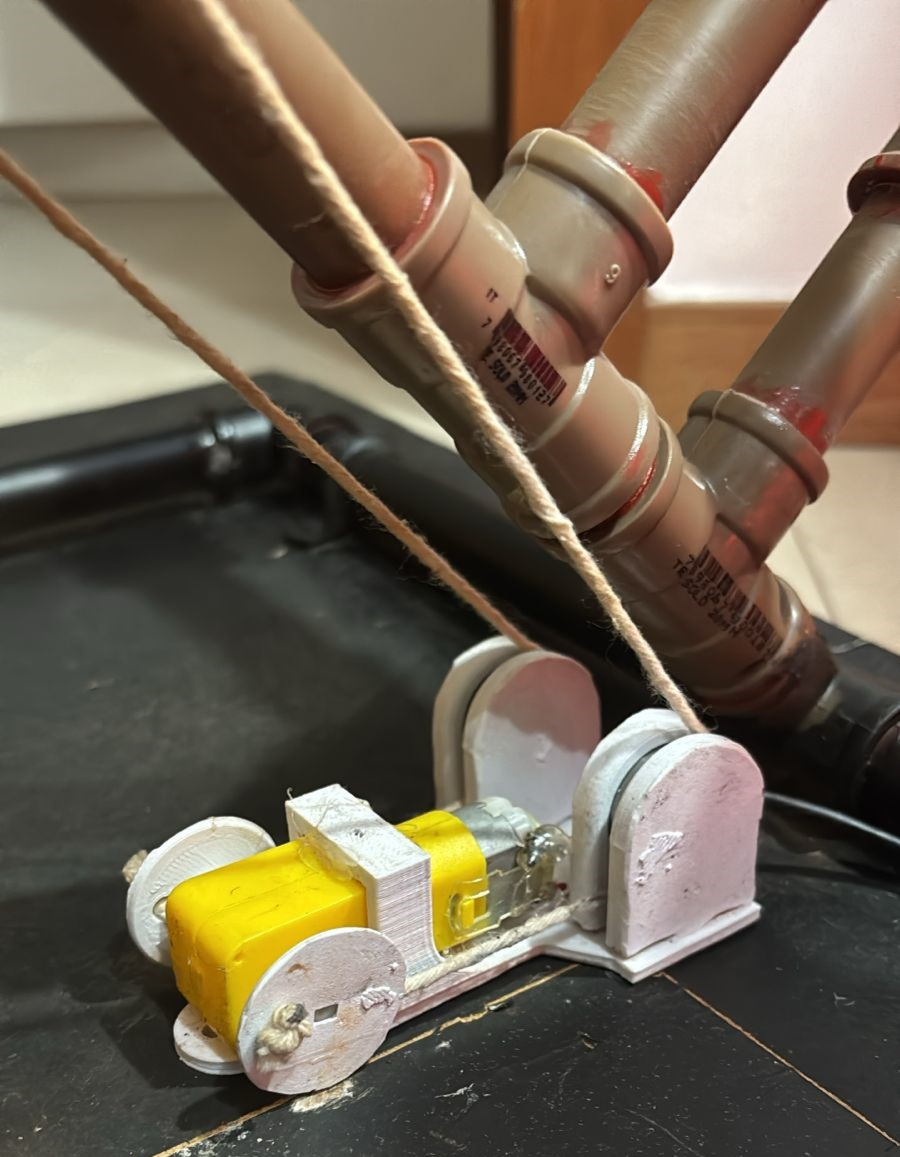
\includegraphics[width=0.5\textwidth,height=\textheight,keepaspectratio]{figuras/estruturas/base_foguete_perto.png}
	\caption{Elementos de filamento ABS na base do foguete.}
	\label{fig_base_foguete_lancamento}
\end{figure}

Para a materialização do projeto, a estrutura de lançamento foi construída majoritariamente com canos e conexões de PVC de 20 mm, enquanto um pedaço de cano de 40 mm foi utilizado para o anel deslizante do mecanismo de gatilho. A base possui um "painel de controle" composto por um braço horizontal que acomoda o manômetro para leitura da pressão e o registro de segurança para alívio do sistema, apresentados na Fig. 4. A pressurização é realizada por meio de uma válvula de bicicleta acoplada à estrutura, conforme a Fig. 5. Esta montagem de PVC é fixada sobre a fundação de suporte retangular de madeira que serve de alicerce e garante a estabilidade do conjunto. 

\begin{figure}[H]
	\centering
	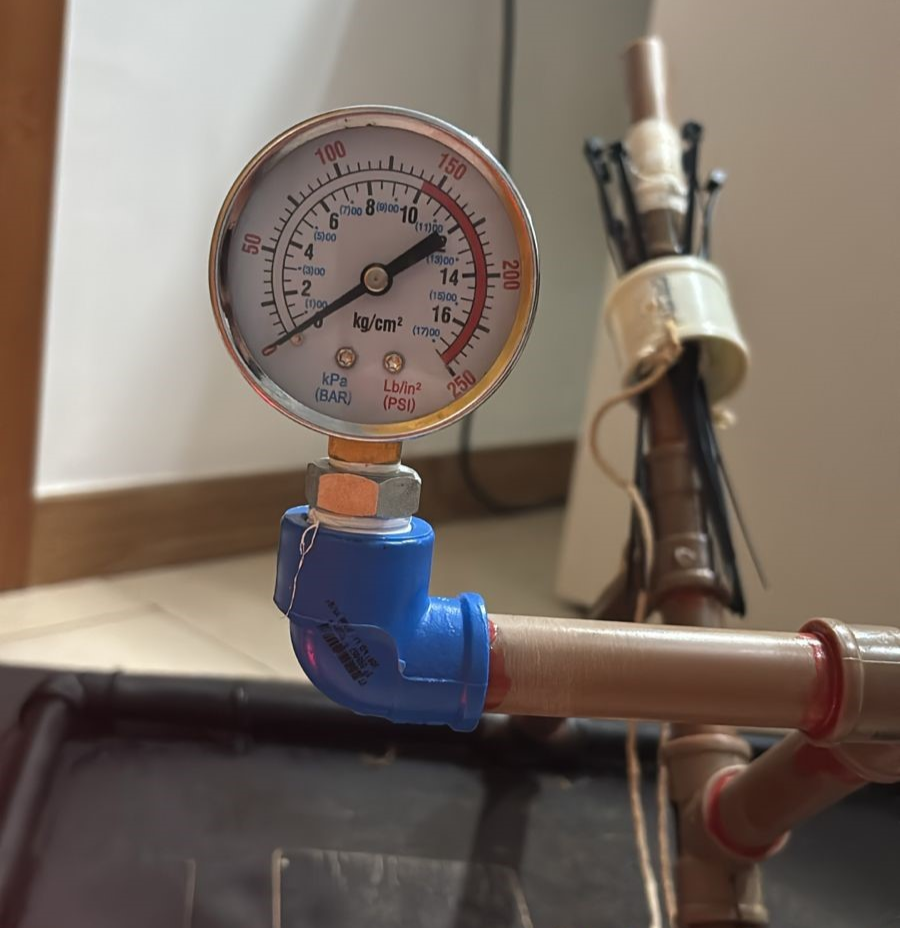
\includegraphics[width=0.75\textwidth,height=\textheight,keepaspectratio]{figuras/estruturas/pressurizador.png}
	\caption{Manômetro acoplado na base para averiguar a pressão aplicada no foguete. }
	\label{fig_pressurizador_foguete}
\end{figure}

\begin{figure}[H]
	\centering
	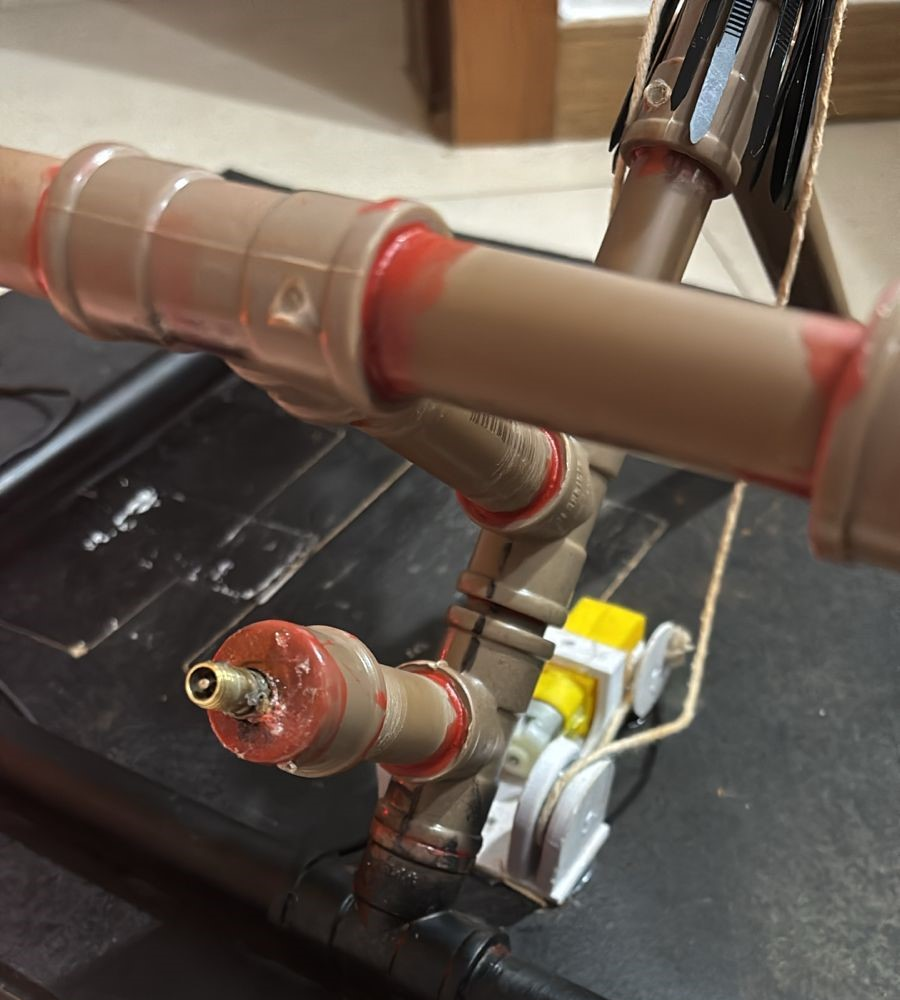
\includegraphics[width=0.75\textwidth,height=\textheight,keepaspectratio]{figuras/estruturas/valvula.png}
	\caption{Válvula usada para pressurização da água.}
	\label{fig_valvula_foguete}
\end{figure}

Para atender ao requisito de automação, o sistema de acionamento consiste em um mecanismo eletromecânico. Este sistema é composto por um servo motor que, por meio de um mecanismo de polia para redirecionamento de força, aciona o gatilho via um barbante. A integração deste sistema exigiu a manufatura de peças customizadas, como o já mencionado case de proteção para o servo motor. Adicionalmente, o hardware de controle foi alojado em um contêiner plástico hermético para proteção contra umidade, poeira e outros possíveis tipos de agentes danosos. 

\subsection{Definição das Aletas}

As aletas exercem um papel fundamental na estabilidade aerodinâmica de foguetes. Sua principal função é deslocar o centro de pressão (CP) para uma posição abaixo do centro de massa (CM), garantindo assim a correção de ângulos de ataque indesejados durante o voo \cite{barrowman1966}. Para cumprir esse papel de forma eficaz, é essencial que as aletas sejam construídas com materiais que combinem baixa densidade, elevada rigidez e espessura reduzida, de modo a minimizar o peso e a interferência aerodinâmica. 

Ademais, a resistência mecânica do material é um fator determinante, uma vez que o foguete está sujeito a impactos significativos durante o pouso. Após analisar diferentes opções, optamos pelo poliestireno de alto impacto (PSAI) para a fabricação das aletas, por oferecer um bom equilíbrio entre rigidez, peso e resistência ao impacto. 

Outros materiais, como o PVC rígido ou plásticos leves de engenharia, também foram considerados, entretanto o PSAI se mostrou mais adequado para o projeto. A escolha inadequada do material poderia levar a deformações durante o voo ou fraturas nas aletas, comprometendo a trajetória e a reutilização do foguete. 

Dessa forma, a definição do material das aletas considerou não apenas o desempenho aerodinâmico, mas também a integridade estrutural ao longo de múltiplos lançamentos, garantindo que o projeto atenda aos requisitos de estabilidade e durabilidade. 

Para garantir uma boa estabilidade durante os lançamentos, foi desenvolvido um modelo computacional do foguete no software OpenRocket a fim de definir o formato e as dimensões das aletas. O programa calcula as posições do centro de gravidade (CG) e do centro de pressão com base na geometria e na massa dos componentes inseridos, fornecendo a margem estática do veículo em calibres (cal). 

O objetivo da análise no OpenRocket foi buscar uma geometria compacta, a fim de minimizar a probabilidade de fratura durante os impactos dos lançamentos, e ainda alcançar uma margem estática satisfatória ligeiramente acima de 1 cal, conforme as recomendações de Barrowman \cite{barrowman1966}. Para atingir a estabilidade necessária com uma boa margem de segurança, foram adicionados 20g como lastro na ponta da coifa, a fim de subir levemente o CG. A figura \ref{fig_foguete_software} mostra o modelo final no OpenRocket, onde observa-se a configuração otimizada e o cumprimento da margem estática estabelecida. A geometria final das aletas, projetada para alcançar estes resultados, está detalhada na figura \ref{fig_atleta}.

\begin{figure}[H]
	\centering
	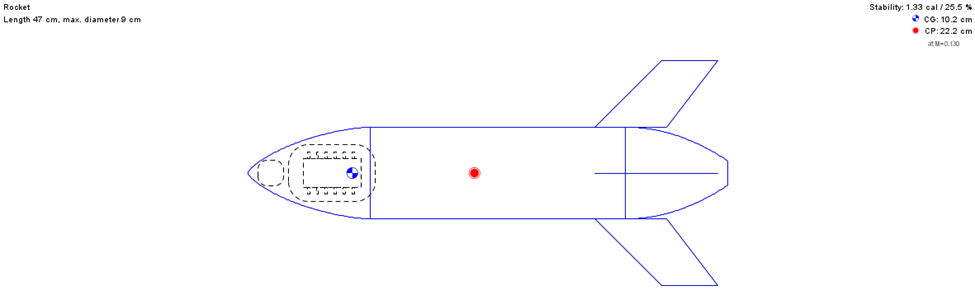
\includegraphics[width=0.75\textwidth,height=\textheight,keepaspectratio]{figuras/estruturas/foguete_software.png}
	\caption{Modelo do foguete no software OpenRocket com a geometria final das aletas.}
	\label{fig_foguete_software}
\end{figure}

\begin{figure}[H]
	\centering
	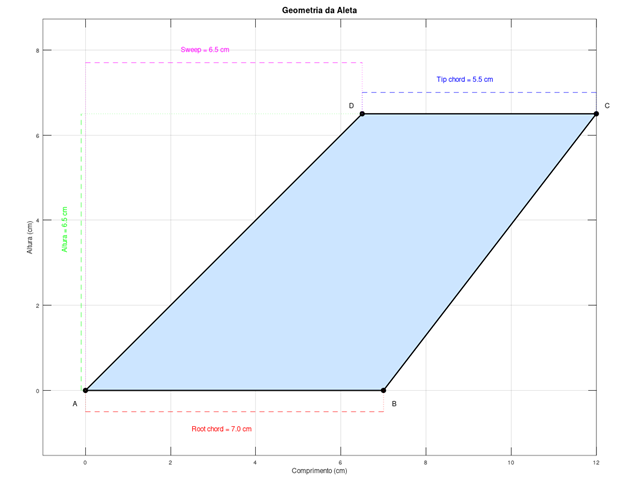
\includegraphics[width=0.75\textwidth,height=\textheight,keepaspectratio]{figuras/estruturas/atleta.png}
	\caption{Dimensões definitivas da aleta.}
	\label{fig_atleta}
\end{figure}

\subsection{Fabricação das Aletas}

A fabricação das aletas foi realizada manualmente a partir de uma placa de PSAI com 1,8mm de espessura, previamente adquirida para o projeto. Utilizando uma régua e um marcador permanente, as quatro aletas foram desenhadas diretamente sobre a superfície da chapa, com base nas dimensões obtidas no modelo do OpenRocket. Esse procedimento garantiu precisão geométrica e invariância entre as peças. 

O corte foi feito com um arco de serra (cegueta), ferramenta adequada para o trabalho com plásticos rígidos, permitindo um controle razoável sobre o contorno mesmo em geometrias trapezoidais. Após o recorte, todas as bordas das aletas foram lixadas cuidadosamente, removendo rebarbas e pequenas imperfeições causadas pelo corte. Esse processo foi essencial para melhorar o acabamento superficial, garantir simetria entre as peças e reduzir o arrasto aerodinâmico. 

A execução manual exigiu atenção aos detalhes para assegurar que todas as aletas mantivessem dimensões idênticas e bom acabamento, fatores indispensáveis para a estabilidade do foguete durante o voo. Além disso, o lixamento contribuiu para reduzir pontos de concentração de tensão, aumentando a resistência mecânica das aletas contra fraturas por impacto durante o pouso. 

\subsection{Desenho Técnico}

A elaboração do desenho técnico utilizando modelagem 3D constituiu uma etapa essencial do projeto, o que permitiu ao grupo a visualização prévia do foguete e sua base de lançamento. Por conta disso ajudou a identificação de possíveis incompatibilidades dimensionais antes da construção física, evitando desperdício de materiais e tempo.

O modelo tridimensional foi desenvolvido no software CATIAV5R21, utilizando as dimensões reais dos componentes selecionados. Para maior precisão, algumas peças padronizadas foram importadas diretamente do repositório TraceParts, mantendo as proporções adequadas (diâmetro de 20mm). Todas as dimensões nas figuras técnicas são expressas em milímetros.


\begin{figure}[H]
	\centering
	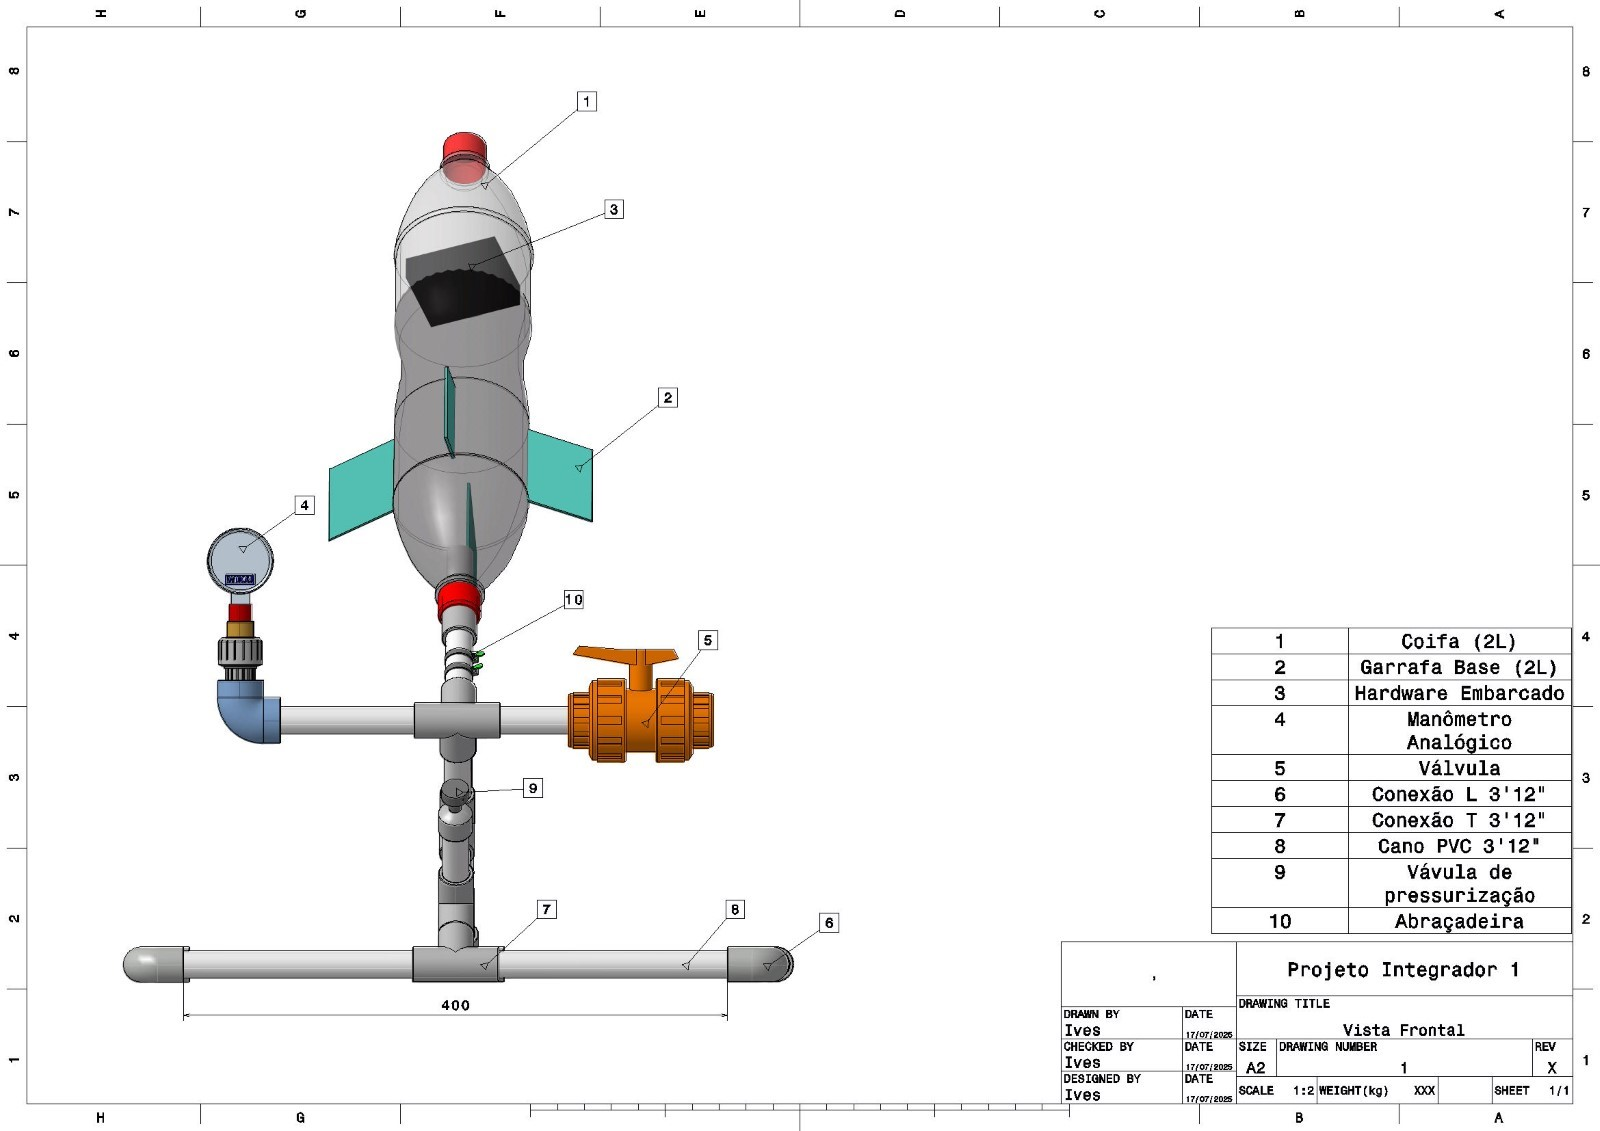
\includegraphics[width=1\textwidth,height=\textheight,keepaspectratio]{figuras/estruturas/foto_modelo_medidas.jpg}
	\caption{Vista frontal do modelo 3D do foguete.}
	\label{fig_foguete_medidas}
\end{figure}

\begin{figure}[H]
	\centering
	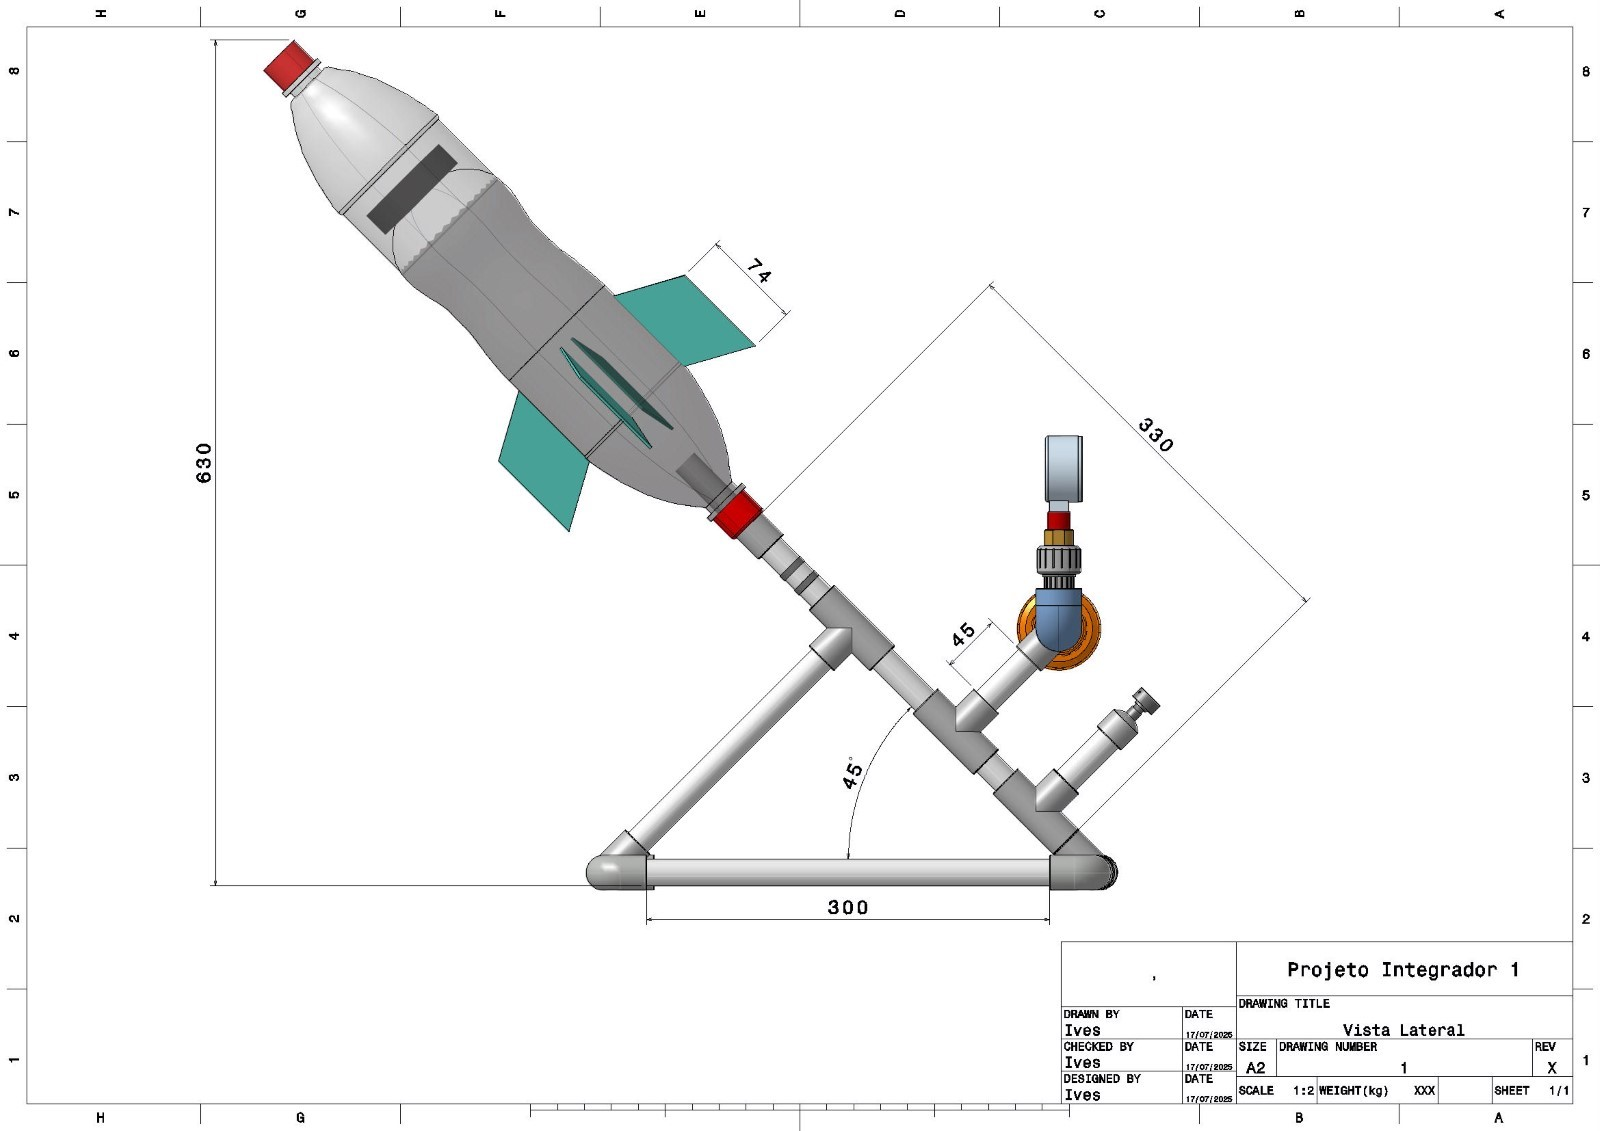
\includegraphics[width=1\textwidth,height=\textheight,keepaspectratio]{figuras/estruturas/modelo_medidas_lado.jpg}
	\caption{Vista lateral do modelo 3D do foguete.}
	\label{fig_foguete_medidas_lado}
\end{figure}


\begin{figure}[H]
	\centering
	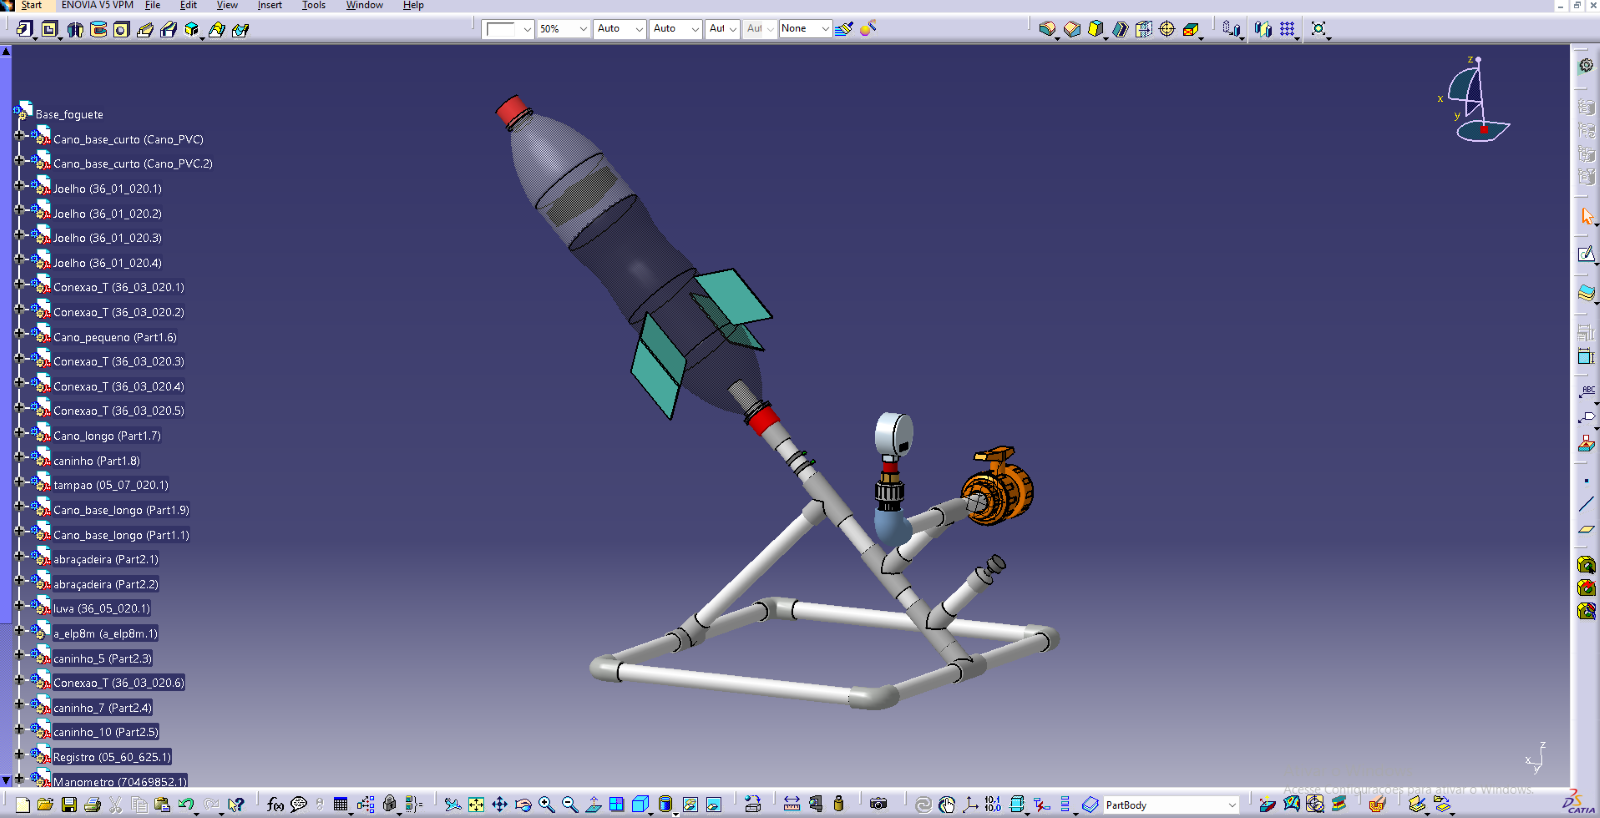
\includegraphics[width=1\textwidth,height=\textheight,keepaspectratio]{figuras/estruturas/desenho_tecnico_catia.png}
	\caption{Desenho Técnico no software CATIAV5R21.}
	\label{fig_desenho_tecnico_catia}
\end{figure}

\subsection{Testes Físicos}

Para assegurar que o material selecionado para a estrutura do foguete suportasse os impactos inerentes ao lançamento e pouso, foi conduzida uma série de testes experimentais simulando quedas controladas. O foco principal foi avaliar a tenacidade e a capacidade de absorção de energia de diferentes tipos de garrafas PET, visando identificar a opção mais adequada para a fuselagem do foguete. 

Para compor a fuselagem do foguete, consideramos duas opções: a garrafa PET convencional e a retornável. Para fins comparativos, uniu-se ambas em um único corpo, conforme ilustrado na figura abaixo. 

\begin{figure}[H]
	\centering
	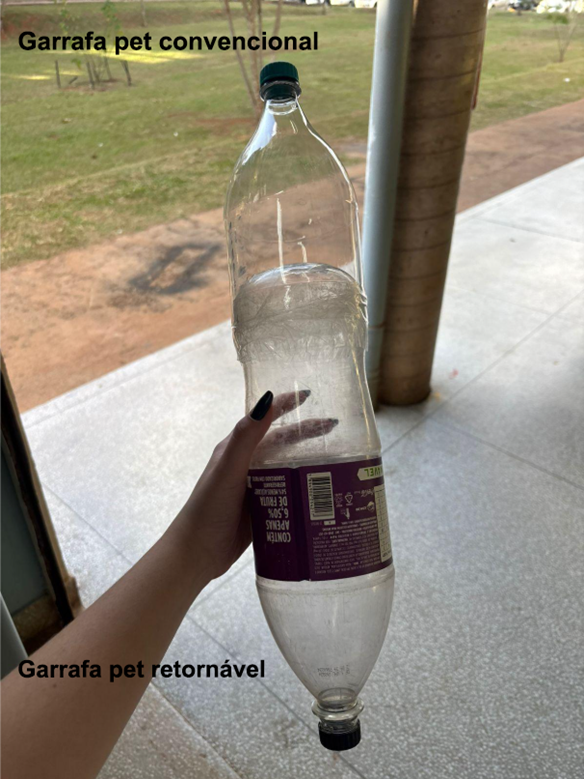
\includegraphics[width=0.4\textwidth,height=\textheight,keepaspectratio]{figuras/estruturas/retornavel_pet.png}
	\caption{Garrafa PET retornável e convencional unidas.}
	\label{fig_garrafa_pet_unidas}
\end{figure}

Com aproximadamente 400 gramas de água adicionados ao interior do foguete, a estrutura foi liberada de cerca de 5 metros de altura. A cada teste, alternou-se a extremidade voltada para o solo, a fim de avaliar a resistência ao impacto de cada material. Essa metodologia permitiu observar a resposta estrutural de ambas as garrafas sob diferentes orientações de impacto. 

\begin{figure}[H]
	\centering
	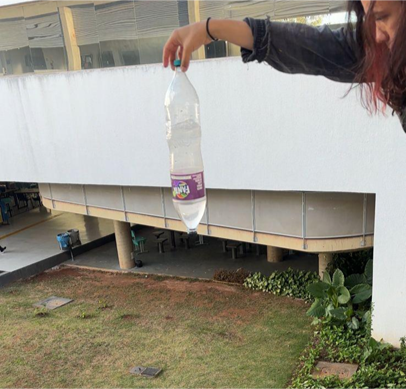
\includegraphics[width=0.4\textwidth,height=\textheight,keepaspectratio]{figuras/estruturas/foto_convencional.png}
	\caption{Garrafa PET retornável e convencional unidas de longe.}
	\label{fig_garrafa_pet_unidas_longe}
\end{figure}

Inicialmente, a garrafa PET retornável foi considerada para a construção da estrutura, devido à sua maior espessura e rigidez. No entanto, observou-se que esse tipo de PET não possui elevada tenacidade; ou seja, tende a romper-se de forma frágil sem apresentar deformação prévia. Além disso, o material perde resistência estrutural com o tempo e o uso repetido. Após algumas quedas, a garrafa PET retornável não resistiu e quebrou, como demonstrado na figura \ref{fig_garrafa_pet_quebrada}.

Em contrapartida, a garrafa PET convencional demonstrou desempenho superior. Apesar de sua menor espessura, ela absorveu os impactos com deformações localizadas que não comprometeram a integridade da estrutura. Essa capacidade de deformação plástica antes da fratura indica uma maior tenacidade, tornando-a mais adequada para aplicações onde a resistência ao impacto é crucial.

\begin{figure}[H]
	\centering
	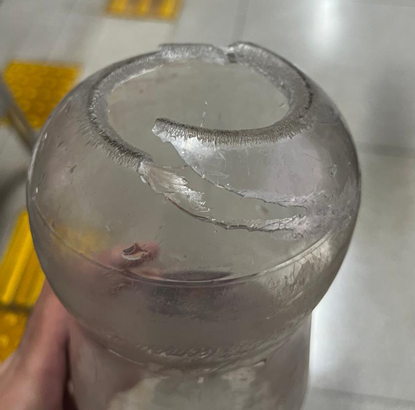
\includegraphics[width=0.5\textwidth,height=\textheight,keepaspectratio]{figuras/estruturas/quebrado.png}
	\caption{Garrafa PET retornável quebrada após os testes.}
	\label{fig_garrafa_pet_quebrada}
\end{figure}

O teste realizado evidenciou que, embora a garrafa PET retornável apresenta maior rigidez, sua baixa tenacidade e suscetibilidade à fratura frágil a tornam menos adequada para a estrutura do foguete. Por outro lado, a garrafa PET convencional, com sua capacidade de absorver energia via deformações plásticas, oferece uma solução mais resiliente e segura para a fuselagem, sendo assim no final para prosseguir com o projeto.

Após a definição dos materiais a serem usados na confecção do foguete, iniciamos testes para não só para determinar a quantidade ideal de água e pressão para atingir as metas, mas também testes para validar a resistência a altas pressões que a sabe será submetida durante os lançamentos, como representado na figura \ref{fig_base_lancamento_perto}.

\begin{figure}[H]
	\centering
	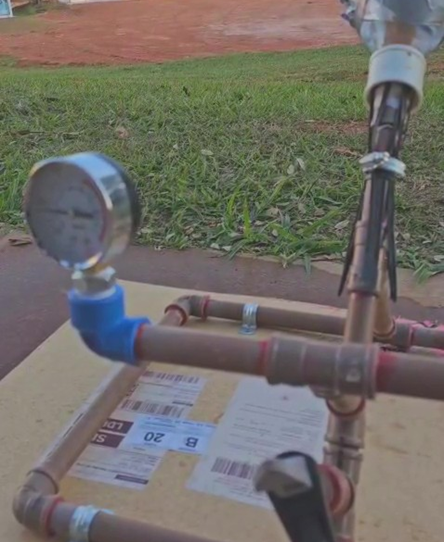
\includegraphics[width=0.5\textwidth,height=\textheight,keepaspectratio]{figuras/estruturas/base_perto.png}
	\caption{Base de lançamento do foguete.}
	\label{fig_base_lancamento_perto}
\end{figure}

Observou-se que pressões muito altas podem causar descarga de água antes do ar alcançar pressão desejada, desperdiçando energia, e para mitigar esse problema foi diminuída a pressão de cada lançamento e implementou-se o uso de veda rosca para a melhor fixação do foguete e diminuir a margem de erro referente ao desperdício de água. 

Quanto à meta de 10 metros, foi averiguado que a base não era capaz de lançar o foguete usando apenas 1 bar de pressão ou menos. Para contornar essa dificuldade, foi adotado o uso de um lubrificante (WD-40) para facilitar o disparo a baixas pressões, assim possibilitando o lançamento. 

Para não comprometer a eletrônica do foguete desnecessariamente, foi utilizado um peso que simulasse sua massa, assim preservando a integridade dos componentes de hardware e garantindo simulações fidedignas no que diz respeito ao caso de voos válido. 

Após o período de de testes e lançamentos para averiguar a acurácia do foguete, foram obtidos os seguintes resultados:

\begin{table}[H]
\centering
\setlength{\tabcolsep}{4pt}
\caption{Tabela de Resultados dos Lançamentos}
\begin{tabular}{|l|p{8cm}|l|}
\hline
Quantidade de água (g) & Pressão aplicada (bar) & Distância (m) \\
\hline
100 & 1 & 10 \\
\hline
150 & 1,5 & 20 \\
\hline
200 & 2 & 30 \\
\hline
\end{tabular}
\label{tab:resultados_lancamentos}
\end{table}